%%%%%%%%%%%%%%%%%
%%%%%%%%%%%%%%%%%
\begin{frame}
	\shiftedframetitle{3. Implementation}
%\vspace{2.5cm}
\begin{minipage}{0.45\textwidth}
\centering
 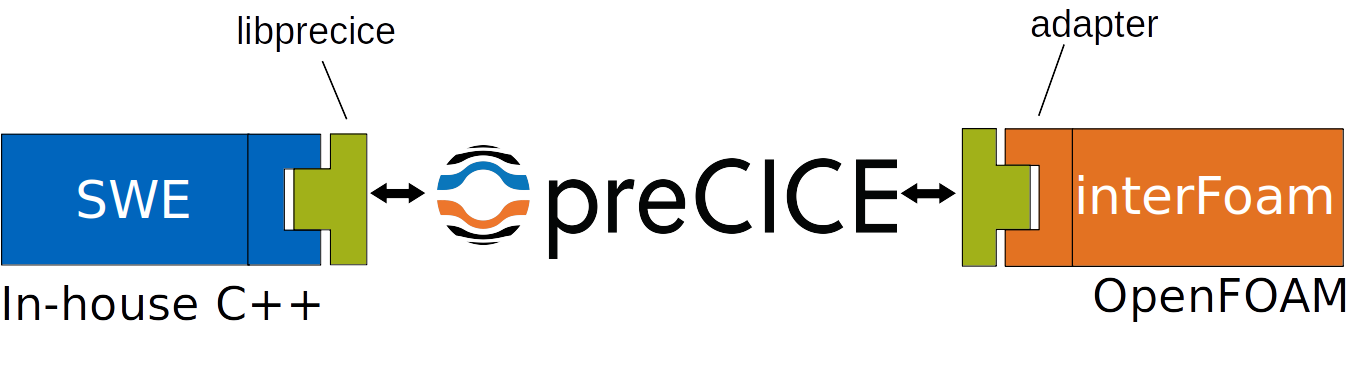
\includegraphics[width=1\textwidth]{Resources/Images/pash2.png}
\end{minipage}
\hspace{1cm}
\begin{minipage}{0.42\textwidth}
\begin{itemize}
\item<2->[]
\begin{tcolorbox}[coltitle=white,title= \textbf{Domain-mapping cases},colframe=black, colback=white] 
\vspace{0.5cm}
\begin{enumerate}
\setlength{\itemsep}{0.1cm}
\item[] \textbf{Left Domain} \qquad  \textbf{Right Domain}
\item[] \par\noindent\rule{0.85\textwidth}{0.5pt}
\item[] $2D$ SWE  \qquad \quad  \ding{222} \quad $2D$  SWE 
\setlength{\itemsep}{1cm}
\item[] {\only<3>{\color{TUMDarkBlue}}$2D$ SWE  \qquad \quad \ding{222}  \quad$3D$ OpenFOAM}   
\item[] {\only<3>{\color{TUMDarkBlue}}$3D$ OpenFOAM   \ding{222} \quad   $2D$ SWE}
\item[] $3D$ OpenFOAM   \ding{222} \quad  $3D$  OpenFOAM
\setlength{\itemsep}{0.05cm}
\item[] \par\noindent\rule{0.85\textwidth}{1.5pt} 
\item[] \quad  \textbf{8 cases in total \quad \footnotesize{(sub \& supercritical)}}
\end{enumerate}
\end{tcolorbox}
\end{itemize}
\end{minipage}
\end{frame}

%%%%%%%%%%%%%%%%%
%%%%%%%%%%%%%%%%




%%%%%%%%%%%%%%%%%%
%%%%%%%%%%%%%%%%%%
%\begin{frame}
%	\shiftedframetitle{3. Implementation}
%
%\begin{minipage}{0.28\textwidth}
% 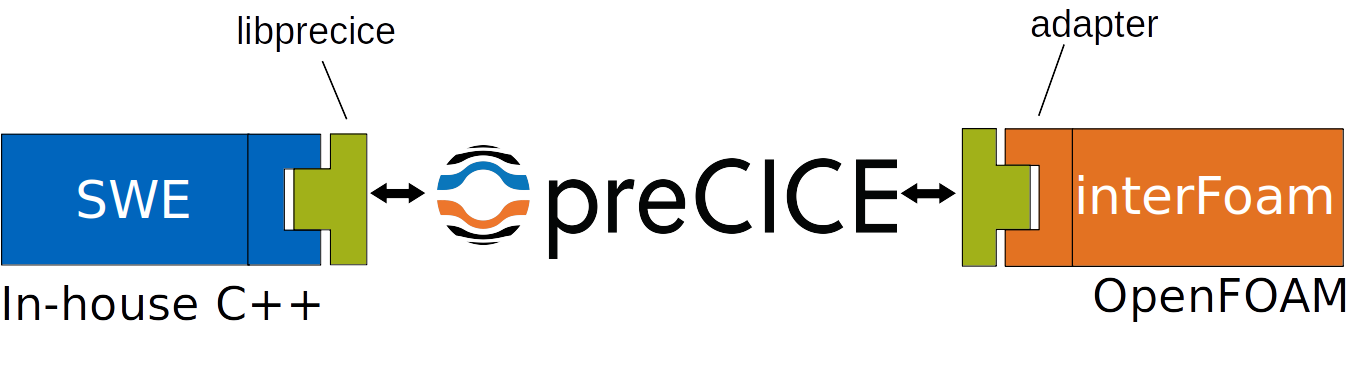
\includegraphics[width=1\textwidth]{Resources/Images/pash2.png}
%\end{minipage}
%\hspace{-0.6cm}
%\begin{minipage}{0.7\textwidth}
%\begin{itemize}
%\item<2->[]
%\begin{tcolorbox}[title= \textbf{Domain Mapping Combinations},colback=white] 
%\begin{table}[]
%\begin{tabular}{llp{0.3cm}ll}
%\textbf{1.} Supercritical & $2D$ SWE  $\rightarrow$  $2D$  SWE  & & \textbf{5.} Supercritical & $3D$ OF   $\rightarrow$  $2D$ SWE  \\ 
%\textbf{2.} Subcritical   & $2D$ SWE  $\rightarrow$  $2D$  SWE & & \textbf{6.} Subcritical   & $3D$ OF   $\rightarrow$  $2D$ SWE     \\[0.2cm]
%\textbf{3.} Supercritical & $2D$ SWE  $\rightarrow$  $3D$  OF   & & \textbf{7.} Supercritical & $3D$ OF   $\rightarrow$  $3D$ OF    \\ 
%\textbf{4.} Subcritical   & $2D$ SWE  $\rightarrow$  $3D$  OF & & \textbf{8.} Subcritical   & $3D$ OF   $\rightarrow$  $3D$ OF
%\end{tabular}
%\end{table}
%\end{tcolorbox}
%\end{itemize}
%\end{minipage}
%
%
%\begin{itemize}
%\item<3->[]
%\begin{tcolorbox}[title= \textbf{Scenarios}, colback=white] 
%\begin{table}[!h]
%\centering
%\begin{tabular}{l|ll|ll}
% & {\large \textbf{Supercritical}} & & {\large \textbf{Subcritical}} &\\[0.3cm]
%\textbf{Case / Domain} & \textbf{Left domain} & \textbf{Right domain} & \textbf{Left domain} & \textbf{Right domain}\\[0.3cm]
%\textbf{SWE $\rightarrow$ SWE} & Radial breaking dam      & Surface at rest   & Radial breaking dam      & Radial breaking dam     \\[0.1cm]
%\textbf{SWE $\rightarrow$ OF}  & Radial breaking dam x2   & Surface at rest & Flow to the right & Surface at rest with wall     \\[0.1cm]
%\textbf{OF $\rightarrow$ SWE}  & Radial breaking dam   & Surface at rest & Flow to the right & Surface at rest with wall   \\[0.1cm]
%\textbf{OF $\rightarrow$ OF}   & Breaking dam      & Empty domain & Breaking dam      & Empty domain with wall
%\end{tabular}
%\end{table}
%\end{tcolorbox}
%\end{itemize}
%\end{frame}

%%%%%%%%%%%%%%%%%%
%%%%%%%%%%%%%%%%%
%\begin{frame}
%%TODO improve this slide
%\shiftedframetitle{3. Implementation}
%\begin{table}[!ht]
%%\hspace{7cm}
%\centering
%\begin{tabular}{ccc}
%\textbf{Boundary Conditions} & & \\
%\hline
%                    				  &$ h$ and $q$ on $\Gamma_{2D}$ & $\alpha, p$ and $u$ on $\Gamma_{3D}$ \\ \hline
%%Supercritical \& Subcritical \case{SWE}{SWE}  & $\begin{aligned}[t] h_{left} &= h_{left} + \partial{h}/\partial{n} \\  hu_{left} &= hu_{left} + \partial{hu}/\partial{n}\\  hv_{left} &= hv_{left} + \partial{hv}/\partial{n} \end{aligned}$ &                  \\ \hline
%%% Subcritical \case{SWE}{SWE}  & $\begin{aligned}[t] \qquad h_{left} = h_{left} + \partial{h}/\partial{n} \end{aligned}$ &                  \\ \hline
%\myTUMdarkblue{Supercritical} \myTUMdarkblue{SWE $\rightarrow$ OF}  & $\begin{aligned}[t] \myTUMdarkblue{\partial{h}/\partial{n} = 0} \\ \myTUMdarkblue{\partial{q}/\partial{n} = 0} \end{aligned}$                 &  $\begin{aligned}[t] \myTUMdarkblue{\alpha = f(h)} \\ \myTUMdarkblue{\partial{p}/\partial{n} = 0}  \\ \myTUMdarkblue{u = f(q,u)}   \end{aligned}$   \\ \hline
%Subcritical \case{SWE}{OF}  & $\begin{aligned}[t] h = \hthD \\ \partial{q}/\partial{n} = 0 \end{aligned}$&    $\begin{aligned}[t] \partial{\alpha}/\partial{n} = 0 \\ \partial{p}/\partial{n} = 0 \\ u = f(q,u) \end{aligned}$              \\ \hline
%Supercritical   \case{OF}{OF}  &$\begin{aligned}[t] h=\hthD \\ q=\qthD \end{aligned}$                                  & $\begin{aligned}[t] \partial{\alpha}/\partial{n} = 0 \\ \partial{p}/\partial{n} = 0 \\ \partial{u}/\partial{n} = 0 \end{aligned}$                      \\ \hline
%Subcritical  \case{OF}{SWE} & $\begin{aligned}[t] \partial{h}/\partial{n} = 0 \\ q=\qthD \end{aligned}$                 &  $\begin{aligned}[t] \partial{\alpha}/\partial{n} = 0 \\ p = f(h) \\ \partial{u}/\partial{n} = 0 \end{aligned}$                \\ \hline
%Supercritical  \case{OF}{OF} &   &  $\begin{aligned}[t] \alpha_{right} = \alpha_{left} \\ u_{right} = u_{left} \\ p_{left} = p_{right} \end{aligned}$                \\ \hline
%%Subcritical   \case{OF}{OF}  & &     \textit{discussion in Section \ref{sec:resultsOFOF}}   \\ \hline
%\end{tabular}
%%\caption{Dirichlet and Neumann boundary conditions for the inter-dimensional combinations and flow characterization \cite{mintgen}, and for the cases on the same dimension.}
%\end{table}
%\end{frame}

%%%%%%%%%%%%%%%%%
%%%%%%%%%%%%%%%%
%\begin{frame}
%\shiftedframetitle{3. Implementation}
%\begin{table}[]
%\begin{tabular}{p{3.5cm}p{4.8cm}p{1cm}p{5cm}}\hline
%                        & \myTUMdarkblue{\textbf{SWE}} & & \myTUMorange{\textbf{interFoam}} \\\hline
%\textbf{Framework}	   & &\\
%					   & SCCS in-house &	& \\
%                        & C++ solver  & & \\\hline
%\textbf{Description}    & \textbf{}    & & \textbf{}          \\
%                        & Riemann Problem solver    &      &        \\
%                        & \textit{F-Wave Method}   		  &      &               \\\hline
%\textbf{Main variables} & \textbf{}    & & \textbf{}          \\
%                        & height  $\rightarrow h$     & &            \\
%                        & velocity $\rightarrow u, v$    &  &      \\
%                        & discharge $\rightarrow hu, hv$        &     &       \\ \hline
%\textbf{Using preCICE}  & & & \\
%					   & build preCICE adapter from scratch & &    \\
%					   
%\end{tabular}
%\end{table}
%\end{frame}


%%%%%%%%%%%%%%%%%
%%%%%%%%%%%%%%%%
\begin{frame}
%TODO improve this slide
\shiftedframetitle{3. Implementation}
\begin{table}[]
\begin{tabular}{p{3.5cm}p{4.8cm}p{1cm}p{5cm}}\hline
                        & \myTUMdarkblue{\textbf{SWE}} & & \myTUMorange{\textbf{interFoam}} \\\hline
\textbf{Framework}	   & &\\
					   & SCCS in-house &	& OpenFOAM\\
                        & C++ solver  & & \\\hline
\textbf{Description}    & \textbf{}    & & \textbf{}          \\
                        & Riemann Problem solver    &      & Free-surface solver        \\
                        & \textit{F-Wave Method}   		  &      & \textit{Volume-of-Fluid Method }               \\\hline
\textbf{Main variables} & \textbf{}    & & \textbf{}          \\
                        & height  $\rightarrow h$     & & volume indicator $\rightarrow \alpha$              \\
                        & velocity $\rightarrow u, v$    &  &pressure    $\rightarrow P$       \\
                        & discharge $\rightarrow hu, hv$        &     & velocity  $\rightarrow u,v,w$       \\ \hline
\textbf{Using preCICE}  & & & \\
					   & build preCICE adapter from scratch & & extend existing preCICE adapter for OpenFOAM   \\
					   
\end{tabular}
\end{table}
\end{frame}

%%%%%%%%%%%%%%%%%
%%%%%%%%%%%%%%%%
\begin{frame}
\shiftedframetitle{3. Implementation}
\begin{minipage}{0.5\textwidth}
\centering
\Large \underline{Supercritical} $2D$ SWE  \ding{222}  $3D$ OpenFOAM 
\end{minipage}
\hspace{4cm}
\begin{minipage}{0.21\textwidth}
\vspace{-1.5cm}
{\scriptsize
\begin{tcolorbox}[colframe=black, colback=white] 
\setlength{\leftmargini}{0pt}
\begin{itemize}
\item[] {\color{black!20}$2D$ SWE  \ding{222}  $2D$ SWE}
\item[] {$2D$ SWE  \ding{222}  $3D$ OpenFOAM} 
\item[]{\color{black!60}$3D$ OpenFOAM   \ding{222}  $2D$ SWE}
\item[] {\color{black!20}$3D$ OpenFOAM   \ding{222}  $3D$ OpenFOAM}
\end{itemize}
\end{tcolorbox}}
\end{minipage}

\hspace{-1cm}
\begin{minipage}{0.2\textwidth}
\vspace{1cm}
\begin{itemize}
\setlength{\leftmargini}{0pt}
\item<2->[]
\begin{figure}
\includegraphics[width=1.1\textwidth]{Resources/Images/imagesThesis/swe_of_sup_schem_top_slides.png}
\caption{Top view}
\includegraphics[width=1.1\textwidth]{Resources/Images/imagesThesis/swe_of_sup_schem_side.png}
\caption{Side view}
\end{figure}
\end{itemize}
\end{minipage}
\hspace{1.3cm}
\begin{minipage}{0.3\textwidth}
\vspace{-0.5cm}
\footnotesize
\begin{itemize}
\setlength{\leftmargini}{0pt}
\item<3->[]
\begin{table}[!ht]
\centering
\begin{tabular}{ccc}
\textbf{Boundary Conditions} & & \\ \\ \hline
  &$ h$ and $q$ on $\Gamma_{2D}$ & $\alpha, p$ and $u$ on $\Gamma_{3D}$ \\\hline
Sup. {SWE $\rightarrow$ OF}  & $\begin{aligned}[t] {\partial{h}/\partial{n} = 0} \\ {\partial{q}/\partial{n} = 0} \end{aligned}$                 &  $\begin{aligned}[t] {\myTUMorange{\alpha = f(h)}} \\ {\partial{p}/\partial{n} = 0}  \\ \myTUMorange{u = f(q,u)}   \end{aligned}$ 
\end{tabular}
\end{table}
\end{itemize}
\end{minipage}
\hspace{2cm}
\begin{minipage}{0.38\textwidth}
\vspace{1cm}
\begin{itemize}
\setlength{\leftmargini}{0pt}
\item<4->[]
\small
\textbf{Volume fraction} ${\alpha_{\Gamma_{3D}}}$
\begin{align*}
 \myTUMorange{\alpha_{\Gamma_{3D}}}\ &=  \begin{cases}
	0, &  \htwD \leq \hthD - 0.5 \Delta \hthD\\
	1, &  \htwD \geq \hthD - 0.5 \Delta \hthD\\
	\dfrac{\htwD-\hthD}{\Delta \hthD} + 0.5, & \text{otherwise}
	\end{cases}
\end{align*}
\textbf{Velocity} $u$
\begin{align*}
 \myTUMorange{\uthD} &= \utwD \ \alpha_{\Gamma_{3D}}
\end{align*}
\end{itemize}
\end{minipage}

\end{frame}



%%%%%%%%%%%%%%%%%
%%%%%%%%%%%%%%%%
\begin{frame}
\shiftedframetitle{3. Implementation}
\begin{minipage}{0.5\textwidth}
\centering
\Large \underline{Subcritical} $3D$ OpenFOAM  \ding{222}  $2D$ SWE 
\end{minipage}
\hspace{4cm}
\begin{minipage}{0.21\textwidth}
\vspace{-1.5cm}
{\scriptsize
\begin{tcolorbox}[colframe=black, colback=white] 
\setlength{\leftmargini}{0pt}
\begin{enumerate}
\item[] {\color{black!20}$2D$ SWE  \ding{222}  $2D$ SWE}
\item[] {\color{black!60}$2D$ SWE  \ding{222}  $3D$ OpenFOAM}  
\item[] {$3D$ OpenFOAM   \ding{222}  $2D$ SWE}
\item[] {\color{black!20}$3D$ OpenFOAM   \ding{222}  $3D$ OpenFOAM}
\end{enumerate}
\end{tcolorbox}}
\end{minipage}

\hspace{-1cm}
\begin{minipage}{0.2\textwidth}
\vspace{1cm}
\begin{itemize}
\setlength{\leftmargini}{0pt}
\item<2->[]
\begin{figure}
\includegraphics[width=1.1\textwidth]{Resources/Images/imagesThesis/of_swe_sub_schem_top_slides.png}
\caption{Top view}
\includegraphics[width=1.1\textwidth]{Resources/Images/imagesThesis/of_swe_sub_schem_side_slides.png}
\caption{Side view}
\end{figure}
\end{itemize}
\end{minipage}
\hspace{1.7cm}
\begin{minipage}{0.3\textwidth}
\vspace{-0.5cm}
\footnotesize
\begin{itemize}
\setlength{\leftmargini}{0pt}
\item<3->[]
\begin{table}[!ht]
\centering
\begin{tabular}{ccc}
\textbf{Boundary Conditions} & & \\ \\ \hline
  &$ h$ and $q$ on $\Gamma_{2D}$ & $\alpha, p$ and $u$ on $\Gamma_{3D}$ \\\hline
Sub.  \case{OF}{SWE} & $\begin{aligned}[t] \partial{h}/\partial{n} = 0 \\  \myTUMdarkblue{q=\qthD} \end{aligned}$                 &  $\begin{aligned}[t] \partial{\alpha}/\partial{n} = 0 \\  \myTUMorange{P = f(h)} \\ \partial{u}/\partial{n} = 0 \end{aligned}$                \\ \hline
\end{tabular}
\end{table}
\end{itemize}
\end{minipage}
\hspace{2.5cm}
\begin{minipage}{0.3\textwidth}
\vspace{2.0cm}
\begin{itemize}
\setlength{\leftmargini}{0pt}
\item<4->[]
\small
\textbf{Discharge} $q_{\Gamma_{2D}}$
\begin{align*}
\myTUMdarkblue{\qtwD} &= \uthD  \hthD(\alpha)
\end{align*}
\textbf{Pressure} ${P}$
\begin{align*}
 \myTUMorange{P_{\Gamma_{3D}}} &= \rho_{\Gamma_{3D}}\ g\ \htwD,\qquad where\\[0.3cm]
\rho_{\Gamma_{3D}} &= \alpha\rho_l + (1-\alpha)\rho_g \\
\end{align*}
\end{itemize}
\end{minipage}

\end{frame}
